\chapter{TF-IDF Outcomes}
\label{ch:tfidfoutcomes}

While it is not really an “achievement,” we were able to get an \~0.116 silhouette score, where 0 means that the distance between clusters is not significant. This means that the closer this number is to 1, the more perfect the clusters are naturally separated. When looking at Cross Validation accuracy, we actually achieved a pretty remarkable 46\% when using a 6-fold configuration. This was calculated using a controlled loop where we tested each configuration of the cross-validation instance to investigate the best fold number to use.

\begin{table}
  \centering
  \label{tab:tfidf_outcomes}
  \begin{tabular}{ | l | r | }
    \hline
    \textbf{Origin} & \textbf{Score} \\
    \hline
    Cross Validation Acc. & 46\% \\
    \hline
    KMeans & 0.116 \\
    \hline
  \end{tabular}
  \caption{Evaluation of TF-IDF Results}
\end{table}

The picture is getting cleared, I hope, on how this is beneficial to instructors as well as students alike. Clustering module content together that relate to one another based on their conveyed topic would not only reduce the scope that students have to be aware of and facilitate a modularized manner of learning.

\begin{figure}
  \centering
  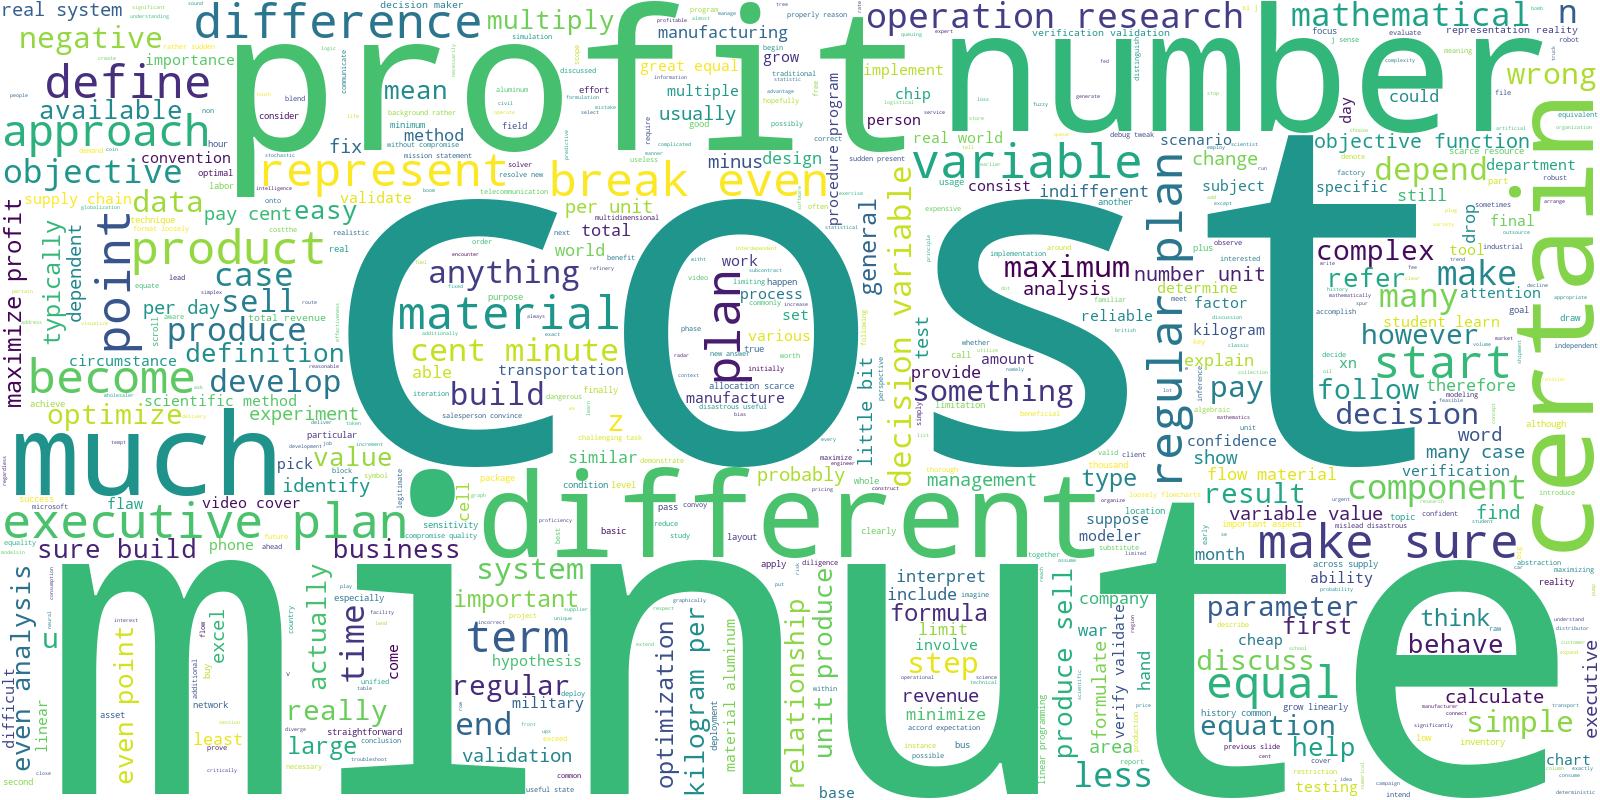
\includegraphics[width=0.6\textwidth]{cluster_0}
  \caption{Word Cloud of TF-IDF Cluster 0}
  \label{fig:tfidf_wordcloud}
\end{figure}
